\section{基于树的回归}
\label{sec:regression-trees}

邻域方法按距离找局部记录，树则按输入条件把空间切成矩形区域，每个区域内给出一个预测。全局线性与局部平滑都假设关系连续渐变，回归树允许在区域交界处发生台阶式跳变，适合关系本身分段、或存在明确条件分支的任务。树规则的基础见第\ref{sec:classic-overview-trees-rules}节。

\subsection{CART回归树}
\label{sec:regression-cart}

\term{分类与回归树}（classification and regression trees, CART）对回归采用递归二分：每次选一个特征与阈值，把当前区域切成两个子区域，叶内输出常数。Breiman、Friedman、Olshen与Stone在1984年把树的生长、最优剪枝与统计性质放在同一体系中\scite{breiman1984cart}。

\subsubsection{模型结构}
\label{sec:regression-cart-structure}

树把输入空间划分为不相交矩形$R_1,\ldots,R_M$，预测为叶常数的分段常数函数
\begin{equation}
  f(\bm{x})=\sum_{m=1}^M b_m\,\mathbb 1\{\bm{x}\in R_m\}.
  \label{eq:regression-cart-model}
\end{equation}
每次分裂只沿一个轴对齐方向，叶内不再区分位置，阈值处可跳跃，新输入沿唯一叶路径到达。

\subsubsection{参数学习}
\label{sec:regression-cart-learning}

\paragraph{树的生长}

枚举特征与合法阈值，节点内叶均值为$b_m=\operatorname{mean}\{y_i:\bm{x}_i\in R_m\}$，叶内平方误差为$\sum_{i\in R_m}(y_i-b_m)^2$。对候选分裂$(j,s)$把$R$分为$R_L,R_R$，用累计统计计算子节点SSE，选择使两侧加权平方误差之和最小的分裂，等价于最大化增益
\begin{equation}
  \Delta(s,j)
  =\sum_{i\in R}(y_i-\bar y_R)^2
   -\sum_{i\in R_L}(y_i-\bar y_L)^2
   -\sum_{i\in R_R}(y_i-\bar y_R)^2.
  \label{eq:regression-cart-gain}
\end{equation}
递归分裂直到叶内样本数、增益或深度达到停止约束。

\paragraph{剪枝与复杂度选择}

无约束生长的树会记住训练波动。代价复杂度给大树加正则：
\begin{equation}
  \mathrm{RSS}(T)+\alpha|T|,
  \label{eq:regression-pruning}
\end{equation}
$|T|$为叶数，$\alpha\geq0$惩罚规模。从$\alpha=0$（完整生长树）开始，逐个剪掉使RSS增加量除以叶数减少量最小的内部分支（即该分支的“弱点”），$\alpha$增大时得到一列嵌套子树；每折重新生长、剪枝，再由验证误差选定$\alpha$与最终树。

\subsubsection{理论分析}
\label{sec:regression-cart-theory}

\paragraph{叶均值与分裂增益}

固定区域$R_m$，对$b_m$求叶内平方误差$\sum_{i\in R_m}(y_i-b_m)^2$的梯度令其为零，得$b_m=\bar y_m$即叶内响应均值，此时叶内SSE为$\sum_{i\in R_m}(y_i-\bar y_m)^2$。一次分裂把$R$分成$n_L,n_R$条记录的左右两叶，两侧叶均值分别为$\bar y_L,\bar y_R$；利用总SSE可分解为“组内SSE$+$组间平方和”，分裂带来的下降恰为
\[
  \Delta(s,j)=\frac{n_L n_R}{n_L+n_R}(\bar y_L-\bar y_R)^2,
\]
即两叶均值差越大、两侧样本越均衡，下降越多；$n_L$或$n_R$为空时该分裂无意义。它只衡量当前节点的局部改善，不保证全局最优划分。

\paragraph{固定生长树上的剪枝最优性}

\begin{theorem}[代价复杂度子树序列]
\label{thm:regression-pruning}
对CART回归树，随$\alpha$增大，使$\mathrm{RSS}(T)+\alpha|T|$最小的最优子树构成有限嵌套序列；每个$\alpha$区间内最优子树不变。
\end{theorem}

\begin{proof}
用归纳证明剪枝递推在固定生长树全部剪枝子树中的最优性：删除一个内部节点把两个叶合并为一个，RSS增加量除以叶数减少量得到该分支的“弱点”$\alpha$；按弱点从小到大剪枝，恰得嵌套序列。该集合是固定生长树的全部剪枝子树，与所有可能的树不同。
\end{proof}

响应参与切分造成选择效应、贪心无法保证全局结构最优及预剪枝可能阻止后续有效切分；低训练SSE不自动控制新样本误差。图\ref{fig:regression-tree-prediction}展示一维树的分段常数预测与训练样本的关系。

\begin{figure}[htbp]
  \centering
  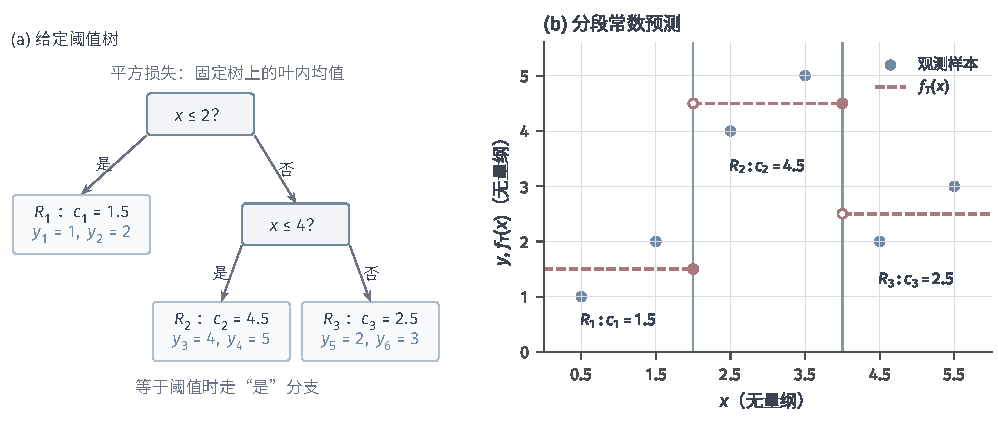
\includegraphics[width=105.412mm]{figures/04-classic-models/00-shared/matplotlib/regression-tree-prediction/figure.pdf}
  \caption{CART回归树的分段常数预测。水平线段为各叶均值，竖线为分裂位置；每个矩形区域内预测取该叶训练响应的平均。}
  \label{fig:regression-tree-prediction}
\end{figure}

\paragraph{支持叶内连续趋势：模型树}
\label{sec:regression-model-tree}

叶内常数忽略了区域内的线性趋势，局部仍有斜率时继续切常数叶要付出代价。\term{模型树}（model tree）在每个叶内拟合一个线性模型：固定分区后，第$m$片叶只用本叶记录最小化
\[
  \sum_{i:\bm{x}_i\in R_m}(y_i-b_m-\bm{w}_m^{\top}\bm{x}_{i,A_m})^2,
\]
用OLS或带正则的线性求解得到系数；新输入先沿树找到叶，再计算该叶的线性预测。若分裂阶段就要按线性叶评价候选，可对每个候选子区域分别重拟合叶模型，比较两侧总残差；此时不能继续把常数叶均值的式\eqref{eq:regression-cart-gain}当成该增益。Quinlan的M5是模型树的代表实现\scite{quinlan1992m5}。叶内样本不足时线性模型不稳定，需加岭惩罚或回退到叶常数；叶与叶之间预测仍按台阶跳跃，相邻叶线性斜率不同会引入额外不连续。分区变量、叶内特征集合与正则强度要和剪枝一起由训练内验证决定，不同模型树实现可采用不同搜索与平滑规则。
